\documentclass[letterpaper, 12pt]{article}

\usepackage{graphicx}
\usepackage{longtable}
\usepackage{rotating}
\usepackage{dcolumn}
\usepackage{listings}
\usepackage{subfiles}
\usepackage{amsmath}

% Code listing commands
\lstset{language=R,
basicstyle=\scriptsize\ttfamily,
commentstyle=\ttfamily,
numbers=left,
numberstyle=\footnotesize,
stepnumber=1,
numbersep=5pt,
showspaces=false,
showstringspaces=false,
showtabs=false,
frame=single,
tabsize=2,
captionpos=b,
breaklines=true,
breakatwhitespace=false,
title=\lstname,
escapeinside={},
keywordstyle={},
morekeywords={}
}

\begin{document}
\title{ARE213 Problem Set \#2B}
\author{Peter Alstone \& Frank Proulx}
\maketitle

\section{Problem \#1}

\subfile{tab-ps2b-1a.tex}
\subfile{tab-ps2b-1b.tex}
\begin{figure}[htbp]
\begin{center}
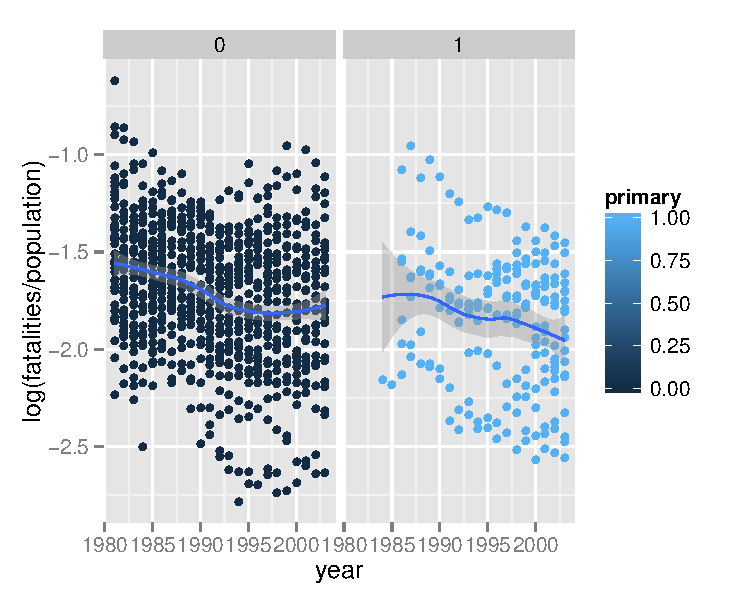
\includegraphics{plot3a.pdf}
\caption{Year to year trends in the log of traffic fatalities per capita, divided by primary seatbelt law presence.  A LOESS fit to each dataset is included for reference but is not necessarily indicative of the true underlying function.}
\label{fig:3a}
\end{center}
\end{figure}

\section{Appendix: Code Listings}

\lstinputlisting{../util/are213-func.R}

\end{document}
